\documentclass[abstract=on,10pt,a4paper,bibliography=totocnumbered]{article}
\usepackage[paper=a4paper,left=35mm,right=35mm,top=25mm,bottom=30mm]{geometry}
\usepackage[doublespacing]{setspace}
\usepackage[english]{babel}
\usepackage[utf8]{inputenc}
\usepackage[round]{natbib}
\usepackage{amsmath}
\usepackage{colortbl}
\usepackage{amsfonts}
\usepackage{amssymb}
\usepackage{gensymb}
\usepackage{graphicx}
\usepackage{tikz}
\usepackage{enumerate}
\usepackage{enumitem}
\usepackage{subcaption}
\usepackage{booktabs}
\usepackage[hidelinks]{hyperref}
\usepackage[nameinlink]{cleveref}
\usepackage{lineno}
\usepackage{multirow}
\usepackage{arydshln}
\usepackage[flushleft]{threeparttable}
\usepackage[nomarkers, nolists]{endfloat}

%------------------------------------------------------------------------------
%	Some Styling
%------------------------------------------------------------------------------
% Creating some TikZ styles
\tikzset{
  nonterminal/.style = {rectangle
    , minimum size = 6mm
    , very thick
    , draw = black!
  }
}

% Changing the style of captions in figures etc.
\captionsetup{labelfont=bf, format=plain, font=small}

% Change how equations are referenced
\renewcommand{\theequation}{Equation \arabic{equation}}%

%------------------------------------------------------------------------------
%	Titlepage: Header
%------------------------------------------------------------------------------
\title{Step by Step: Using Step Selection Analysis to Simulate Dispersal and
Assess Landscape Connectivity}

% List of Authors
\author{
  David D. Hofmann\textsuperscript{1,\S} \and
  John W. McNutt\textsuperscript{2} \and
  Arpat Ozgul\textsuperscript{1} \and
  Gabriele Cozzi\textsuperscript{1,2} \and
  Dominik M. Behr\textsuperscript{1,2}
}

% Reduce spacing between authors
\makeatletter
\def\and{%
  \end{tabular}%
  \hskip -0.5em \@plus.17fil\relax
  \begin{tabular}[t]{c}}
\makeatother

% Current Date
\date{\today}

% And here the masterpiece begins
\begin{document}

% Change page numbering
\pagenumbering{gobble}

% Required to be able to cite
\bibliographystyle{apalike}

% Create Titlepage
\maketitle

%------------------------------------------------------------------------------
%	Titlepage: Additional Info
%------------------------------------------------------------------------------
\begin{flushleft}

\vspace{0.5cm}

\textsuperscript{1} Department of Evolutionary Biology and Environmental
Studies, University of Zurich, Winterthurerstarsse 190, 8057 Zurich,
Switzerland.

\textsuperscript{2} Botswana Predator Conservation, Private Bag 13, Maun,
Botswana.

\textsuperscript{\S} Corresponding author (david.hofmann2@uzh.ch)

\vspace{4cm}

\textbf{Running Title:} Release the Dogs! Simulating Wild Dog Dispersal to
Assess Landscape Connectivity

\vspace{0.5cm}

\textbf{Keywords:} dispersal, simulation, movement, integrated step selection,
Kavango-Zambezi Transfrontier Conservation Area, landscape connectivity, Lycaon
pictus

\end{flushleft}

%------------------------------------------------------------------------------
%	Abstract
%------------------------------------------------------------------------------
\newpage
\begin{abstract}
Dispersal is an important process that allows species to avoid inbreeding, to
colonize new habitats and to reinforce non-viable subpopulations. Successful
dispersal thus represents a crucial pre-requisite for long-term species
persistence in wild animal populations. However, the ability to disperse is
contingent a sufficient degree of landscape connectivity, which is why the
estimation of connectivity and identification of dispersal corridors has become
a task of extraordinary importance in ecological studies.

Over the past two decades, ecologists have primarily relied on analytical tools
such as least-cost methods and circuit theory to investigate landscape
connectivity. Despite their usefulness for various ecological applications, both
methods make several restricting assumptions that limit their suitability in
reality. To address their shortcomings, simulations from individual-based
movement models have been proposed and applied. To overcome their shortcomings,
simulations from individual-based movement models have been proposed. Yet, due
to the infinite number of possibilities of coming up with an individual-based
model, a unified and objective framework is missing.

Recent innovations in movement ecology have brought forward novel opportunities
to study animal dispersal and landscape connectivity. In particular, the rich
suite of resource selection functions, including point-, step-, and
path-selection functions have undergone substantial improvements over the past
years. Most notably, step-selection functions have been generalized to
\textit{integrated} step selection functions, which essentially represent fully
mechanistic movement models based on which individual animal movement could be
simulated. While such models have been applied to study \textit{steady-state}
utilization distribution, a similar approach may be useful for investigating
\textit{transient} movement behavior and thereby study landscape connectivity by
means of simulated dispersal events.

Here, we showcase the use of integrated step selection analysis to simulate
dispersal of the highly endangered African wild dog across the world's largest
transboundary conservation area, the Kavango-Zambezi Transfrontier Conservation
Area (KAZA-TFCA). For this, we utilize data collected on 16 dispersing wild dog
coalitions departing from northern Botswana. We combine the movement data with
relevant spatial covariate layers and used integrated step selection functions
to parametrize a fully mechanistic movement model rendering wild dog dispersal.
Based on this model, we simulate 80'000 dispersers, originating from protected
areas and moving across the extent of the KAZA-TFCA. We then generate a heatmap
and use network theory to reveal dispersal hotspots and crucial bottlenecks
across the study area. Finally, we discuss the benefits and pitfalls of such
dispersal simualtions and highlight potential improvements to be made in the
future.
\end{abstract}

%------------------------------------------------------------------------------
%	Main Text
%------------------------------------------------------------------------------
\newpage

\onehalfspacing
\tableofcontents
\doublespacing

% Change page numbering
\newpage
\pagenumbering{arabic}

% Create linenumbers
\linenumbers

\section{Introduction (90\%)}

% Importance of Dispersal & Connectivity
\subsection{Importance of Dispersal \& Connectivity (90\%)}
Dispersal is defined as the movement of individuals from their natal location to
the site of first reproduction \cite{Howard.1960}. It is a vital process
governing the dynamics wild animal populations that are distributed in space
\citep{Hanski.1998, Clobert.2012} and may strongly affect population dynamics at
different spatial and social scales \citep{Hanski.1999a, Clobert.2012}.
Dispersal allows species to avoid inbreeding and maintain genetic diversity
\citep{Perrin.1999, Perrin.2000, Frankham.2002, Leigh.2012, Baguette.2013}, to
rescue small and non-viable populations \citep{Brown.1977}, and to promote the
colonization of unoccupied habitats \citep{Hanski.1999b, MacArthur.2001}.
However, successful dispersal requires a sufficient degree of functional
connectivity \citep{Fahrig.2003, Clobert.2012}, which is why the identification
and protection of major dispersal corridors has become an important task in
conservation science \citep{Doerr.2011, Rudnick.2012}. To achieve this, reliable
information on movement behavior during dispersal and knowledge about factors
that limit dispersal and connectivity is paramount \citep{Baguette.2013,
Vasudev.2015}.

% Advancements in GPS Technology & Movement Ecology
\subsection{Advancements in GPS Technology \& Movement Ecology (90\%)}
Thanks to novel technologies developed over the past decades, particularly of
GPS/Satellite radio-collars, the use of GPS data to study animal dispersal and
connectivity has accelerated \citep{Elliot.2014, Jonsson.2016, Williams.2019}.
Additionally, the advent of publicly accessible satellite imagery and
sophisticated remote sensing techniques to represent the physical landscape
through which individuals disperse have heralded a ``golden age of animal
tracking'' \citep{Kays.2015}. Concurrently, the availability of large amounts of
empirical data and an increased computational power have led to the development
of numerous techniques to study dispersal movements and highlight critical
corridors between subpopulations \citep{Boyce.2002, Fortin.2005, Cushman.2010,
Zeller.2012, Diniz.2020}.

% Resource Selection & Connectivity
\subsection{Resource Selection \& Connectivity (90\%)}
\textit{Resource selection functions} \citep{Boyce.2002} and derived methods
such as \textit{step selection functions} \citep{Fortin.2005} and \textit{path
selection functions} \citep{Cushman.2010} have proven particularly useful for
studying animal movement \citep{Fieberg.2020} and modelling connectivity
\citep{Diniz.2020}. These methods allow estimating habitat preferences of the
focal species by comparing covariates at locations visited by the animal to the
same covariates at locations available to, but not visited by the animal
\citep{Boyce.2002, Fortin.2005, Cushman.2010, Thurfjell.2014}. The so estimated
preferences can then be used to predict a permeability surface, indicating the
expected ease at which an animal can traverse a given area \citep{Spear.2010,
Zeller.2012, Etherington.2016}. Ultimately, the permeability surface serves as
input to a connectivity model that is used to reveal movement corridors
\citep{Diniz.2020}. Two of the most prominent connectivity models are least-cost
path analysis (LCP analysis; \citealp{Adriaensen.2003}) and circuit theory (CT
\citealp{McRae.2006, McRae.2008}), both graph-based methods that estimate
conductance of the landscape. Despite their intuitive nature and ease of use,
both methods make rigorous assumptions about animal movement that may or may not
be fulfilled in reality \citep{Diniz.2020}.

% Issues with Least-Cost Paths & Circuit Theory
\subsection{Issues with Least-Cost Paths \& Circuit Theory (90\%)}
In LCP analysis, for instance, a least costly path always exists, even if
associated movement costs are unreasonably high and will never be incurred by a
dispersing individual. The method also presumes that animals have an infinite
perceptual range, a preconceived end-point in mind, and choose a cost-minimizing
route accordingly. These assumptions may be reasonable for migrating animals,
yet they are unlikely to be true for dispersers that move over long distances
into unknown territory \citep{Koen.2014, Abrahms.2017, Cozzi.2020}. Finally,
LCPs are only one pixel wide, meaning that their absolute size depends on the
resolution of chosen covariate layers \citep{Diniz.2020}. Although some of these
issues can be alleviated using less stringent versions of the LCP algorithm
(e.g. least-cost \textit{corridors} \citep{Pinto.2009}, \textit{thresholded}
least-cost paths \citep{Landguth.2012}, and \textit{randomized} least-cost paths
\citep{Panzacchi.2016, VanMoorter.2021}), a certain degree of arbitrariness in
the assumptions remains. CT entails similar restrictions. Because CT only
considers movements from the source cell to its 4 or 8 adjacent cells, it
implicitly posits a perceptual range of a single pixel. It is also built on the
assumption of a complete random walk \citep{Diniz.2020}, implying that
directional biases cannot be rendered, albeit being very common in dispersal
movements \citep{Cozzi.2020, Hofmann.2021}. Ultimately, both LCP analysis and CT
omit the temporal dimension of dispersal. In result, statements about the
expected duration required to traverse a certain corridor are impossible.
Because movement is not modelled explicitely, neither of the methods can render
possible interactions between movement behavior and landscape characteristics
such that connectivity mainly arises as a result of the landscape structure.
This is referred to as structural connectivity and stands in contrast to
functional connectivity, which also renders the behavioral response of the
animal with respect to prevailing habitat conditions \citep{Tischendorf.2000}.
Even though functional connectivity is more difficult to estimate, a functional
view is the ultimate goal in conservation science because it has direct
consequences for gene flow \citep{Baguette.2013}.

% What about IBMMs?
\subsection{What about IBMMs? (90\%)}
To address the issues inherent to LCPs and CT, individual-based movement models
(IBMMs) have been proposed and applied \citep{Diniz.2020}. In these models,
dispersal is simulated explicitly, based on movement rules that determine how
individuals move over and interact with the prevailing landscape
\citep{Kanagaraj.2013, Clark.2015, Allen.2016, Hauenstein.2019, Zeller.2020,
Vasudev.2021}. Using the simulated trajectories, one can calculate a set of
connectivity metrics, such as interpatch-connectivity and traversal frequency
across the landscape to reveal major dispersal hotspots \citep{Kanagaraj.2013,
BastilleRousseau.2018, Hauenstein.2019, Zeller.2020}. Even though IBMMS can be
employed to overcome any of the shortcomings intrinsic to LCPs and CT, as well
as to provide a more functional view on connectivity, they can be challenging to
fit and require vast amounts of data collected during dispersal
\citep{Diniz.2020}.

% Step Selection Analysis
\subsection{Step Selection Analysis (90\%)}
Here, we investigate the usefulness of integrated step selection functions
(ISSFs, \citealp{Avgar.2016}), as a relatively simple but powerful IBMM based on
which dispersal can be simulated. While regular SSFs were intended to learn
about relative habitat preferences of the focal species \citep{Fortin.2005,
Thurfjell.2014, Avgar.2017}, the method has been generalized and now enables to
jointly study habitat and movement preferences, as well as potential
interactions between movement and habitat preferences \citep{Avgar.2016,
Signer.2017, Fieberg.2020}. ISSFs therefore provide a relatively simple method
to model complex movement behavior where movement results from two intertwined
behavioral kernels (e.g. \citealp{Prokopenko.2017, Munden.2020}). Importantly, a
parametrized ISSF model can be viewed as a fully mechanistic movement model
based on which individual movement trajectories can be simulated
\citep{Avgar.2016, Signer.2017}. In fact, \cite{Signer.2017} used ISSF to
simulate steady state utilization distributions of resident animals. However,
the degree to which such simulations are helpful in detecting movement corridors
and modeling landscape connectivity is unknown.

% Study Species & Study Area
\subsection{Study Species \& Study Area (90\%)}
One of the species for which long-term viability relies on sufficient
landscape connectivity is the endangered African wild dog \textit{Lycon pictus}.
While once present across entire sub-Saharan Africa, wild dogs have disappeared
from a vast majority of their historic range due to persecution by humans,
habitat destruction, and deadly diseases. As of today, only 6'000 free-ranging
individuals remain in small and spatially scattered subpopulations
\citep{Woodroffe.2012}. Within those subpopulations, wild dogs form cohesive
packs comprising 8 to 12 adults and their offspring \cite{McNutt.1995}. After
reaching sexual maturity, male and female offspring form same-sex coalitions and
disperse from their natal pack \citep{McNutt.1996, Behr.2020}. New packs are
formed when dispersing coalitions join unrelated opposite-sex dispersing
coalitions \citep{McNutt.1996}. Dispersing wild dogs can cover several hundred
kilometers across a variety of landscapes \citep{DaviesMostert.2012,
Masenga.2016, Cozzi.2020, Hofmann.2021}. One of the few strongholds for this
species lies near the Moremi Game Reserve in northern Botswana, which is part of
the world's largest transboundary protected area, namely the Kavango-Zambezi
Transfrontier Conservation Area (KAZA-TFCA). This area has originally been
intended to facilitate migration of elephants, but is expected to benefit a
multitude of other species \citep{Elliot.2014, Brennan.2020, Hofmann.2021}.

% Previous Paper
\subsection{Previous Paper (90\%)}
In a previous study, we assessed landscape connectivity for dispersing African
wild dogs within the KAZA-TFCA using a least-cost corridor approach
\citep{Hofmann.2021}. For this, we fitted a basic habitat selection model based
on which we predicted landscape permeability. We now expand on this knowledge
and use ISSF to develop a more detailed movement model of dispersing wild dogs.
We then use this model to simulate dispersers moving across the KAZA-TFCA. Based
on simulations, we compute heatmaps and identify potential dispersal hotspots.
We also showcase how network metrics relevant to landscape connectivity can be
computed. Our results show that a simulation-based approach yields several major
benefits over traditional connectivity modeling techniques. Most importantly,
simulations provide a more generic view on how connectivity emerges and to which
degree connectivity depends on the dispersal duration. In addtion, by generating
proper dispersal trajectories, network theory can be applied to calculate
network metrics that are pertinent to connectivity analysis. Finally, we put
forward additional opportunities using simulations that go beyond the scope of
this paper.

\section{Methods}
\subsection{Study Area (90\%)}
The study area was centered at -17\degree 13'9''S, 23\degree 56'4''E
(\Cref{StudyArea}a) and was represented by a rectangular bounding box that
stretched over 1.3 Mio. km\textsuperscript{2}, ecompassing the entire KAZA-TFCA
(\Cref{StudyArea}b). The KAZA-TFCA is the world's largest transboundary
conservation area and comprises parts of Angola, Botswana, Namibia, Zimbabwe,
and Zambia, covering a total of 520'000 km\textsuperscript{2}. Its landscape
varies regionally and ranges from savanna, to grassland and from dry to moist
woodland habitats. A dominant hydrogeographical feature in its center is the
flood-pulsing Okavango Delta. The wet season within the KAZA-TFCA lasts from
November to March and is out of phase with the main flooding of the Okavango
Delta which peaks between July and August \citep{McNutt.1996, Wolski.2017}.
While large portions within the KAZA-TFCA are designated national parks or other
protected areas, substantial human influence remains due to roads, agricultural
sites and settlements and villages.

\begin{figure}[htbp]
  \begin{center}
    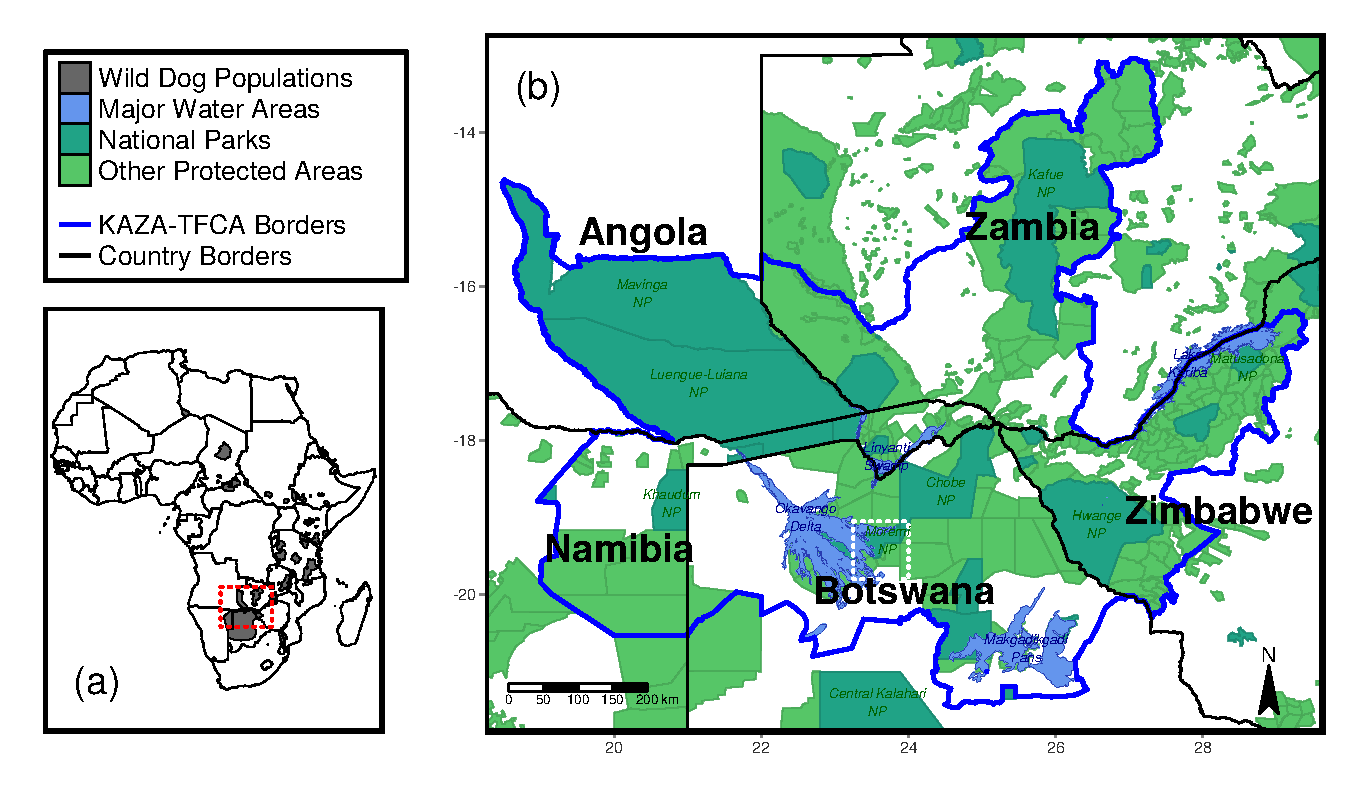
\includegraphics[width = \textwidth]{99_StudyArea.png}
    \caption{(a) The study area was confined by a bounding box encompassing the
    entire KAZA-TFCA and spanned parts of Angola, Namibia, Botswana, Zimbabwe,
    and Zambia. (b) The KAZA-TFCA represents the world's largest terrestrial
    conservation area and covers a total of 520'000 km\textsuperscript{2}. Its
    purpose is to re-establish connectivity between already-existing national
    parks (dark green) and other protected areas (light green). The dispersal
    data used in this study was collected on a free-ranging African wild dog
    population inhabiting the Moremi National Park in northern Botswana.}
    \label{StudyArea}
  \end{center}
\end{figure}

\subsection{GPS Relocation Data (90\%)}
Between 2011 and 2019, we collected GPS relocation data on dispersing wild dogs
from a free-ranging wild dog population inhabiting the Moremi National Park in
northern Botswana. We selected potential dispersers based on age, pack size,
number of same‐sex siblings within the pack, and presence of unrelated
opposite-sex individuals in the pack \citep{McNutt.1996, Behr.2020}. We
immobilized selected individuals using a cocktail of Ketamine/Xylazine/Atropine
\citep{Osofsky.1996, Cozzi.2020} that was injected by dart, fired from a
CO\textsubscript{2}-pressurized gun (\textit{DAN-Inject, Denmark}). Immobilized
individuals were fitted with GPS/Satellite radio collars (\textit{Vertex Lite;
Vectronic Aerospace GmbH, Berlin}) that guaranteed automated drop-off through a
decomposable piece of cotton. Handling and collaring of all individuals was
supervised by a Botswana-registered wildlife veterinarian. All individuals
rejoined their pack within one hour after immobilization. 16 collared
individuals eventually dispersed, each in a separate same-sex dispersal
coalition (7 female and 9 male coalitions).

Because behavior during dispersal is more pertinent for assessing landscape
connectivity \citep{Elliot.2014, Abrahms.2017}, we discarded all data that was
collected during residency and only retained GPS data recorded during dispersal.
During dispersal, collars were programmed to record a GPS fix every 4 hours.
Collected relocations were regularly transmitted over the Iridium satellite
system, which allowed remote tracking of individuals, even if they left the main
study area and crossed international borders. In some instances, exact dispersal
dates were known from field observations. Otherwise, we distinguished between
residency and dispersal using the net-squared displacement metric. This metric
measures the squared Euclidean distance of a GPS relocation to a reference point
\citep{Borger.2012}, which in our case was set to the center of each
individual's natal home range. As such, dispersal was deemed to have started
when an individual left its natal home range and ended once individuals became
sedentary again. As previous research revealed similar behavior of females and
males during dispersal \citep{Woodroffe.2019, Cozzi.2020}, we did not
distinguish between sexes. After collection, we converted collected GPS
coordinates (n = 4'169) to steps, where each step represented the straight-line
distance traveled by and individual between two consecutive GPS relocations
\citep{Turchin.1998}. To ensure a regular sampling interval, we removed fixes
that were not successfully collected on the 4-hourly schedule.

\subsection{Covariates (90\%)}
We represented the physical landscape across the study area using a set of
habitat covariates including water-cover, distance to water, woodland-cover, and
shrub/grassland-cover. Because water cover greatly changes within and between
years in the Okavango Delta, we applied a remote sensing algorithm and generated
frequently updated water cover layers and corresponding distance to water layers
(see \citealp{Wolski.2017} and \citealp{Hofmann.2021}). Resulting layers thus
temporally aligned with our dispersal events. We furthermore computed a proxy
for human influence, depicting anthropogenic pressures stemming from
human-density, agricultural sites, and roads. All spatial layers were coarsened
or interpolated to a target resolution of 250 m by 250 m. Further details on the
sources and preparation of each habitat covariate are given in
\cite{Hofmann.2021}.

Besides habitat covariates, we also computed movement metrics that we used as
movement covariates in our models. Movement metrics were calculated for each
step and included the step length (\textsf{sl}), its natural logarithm
(\textsf{log(sl)}), and the cosine of the relative turning angle
(\textsf{cos(ta)}). Because wild dogs follow a diurnal activity pattern, we also
coded a binary variable (\textsf{LowActivity}) indicating whether a step was
realized during periods of low wild dog activity (17:00 to 07:00 local time) or
high wild dog activity (09:00 to 17:00 local time). Handling and manipulation of
all data, as well as all models and simulations were implemented with the
statistical software {\tt R}, version 3.6.6 \citep{R.2019}. Several helper
functions were written in {\tt C++} and imported into {\tt R} using the {\tt
Rcpp} package \citep{Eddelbuettel.2011, Eddelbuettel.2013}

\subsection{Movement Model (80\%)}
We used ISSFs to parametrize a mechanistic movement model for dispersing wild
dogs \citep{Avgar.2016}. To conduct iSSF analysis, we paired each observed step
with 24 random steps. An observed and its 24 random steps thus formed a stratum
and received a unique identifier. We generated random steps by sampling random
turning angles from a uniform distribution (\(-\pi, +\pi\)) and step lengths
from a gamma distirbution that was fitted to observed steps (scale = 6'308,
shape = 0.37). Along each step, we extracted and averaged spatial covariates
using the {\tt velox}. We also calculated the movement metrics \textsf{sl},
\textsf{log(sl)}, and \textsf{cos(ta)}. To facilitate model convergence, we
standardized all continuous covariates to a mean of zero and a standard
deviation of one. Since correlation among covariates was low (\(|r| > 0.6\);
\citealp{Latham.2011}), we retained all of them for modeling.

To contrast realized steps (scored 1) and random steps (scored 0), we assumed
that animals assigned a selection score \(w(x)\) of the exponential form to each
step. The selection score \(w(x)\) of each step depended on its associated
covariates (\(x_1, x_2, ..., x_n\)) and on the animal's relative selection
strengths (i.e. preferences) towards these covariates (\(\beta_1, \beta_2, ...,
\beta_n\)):

\begin{equation}
\label{EQ1}
  w(x) = exp(\beta_1 x_1 + \beta_2 x_2 + ... + \beta_n x_n)
\end{equation}

The probability of a step being realized was then contingent on the step's
selection score, as well as on the selection scores of all other step in the
same stratum:

\begin{equation}
\label{EQ2}
  P(Y_{i} = 1 | Y_{1} + Y_{2} + ... + Y_{i} = 1) =
  \frac{w(x_{i})}{w(x_{1}) + w(x_{2}) + ... + w(x_{i})}
\end{equation}

To estimate the preferences of interest, we ran conditional logistic regression
models in the r-package {\tt glmmTMB}. To handle multiple individuals, we
applied the mixed effects method developed by \citep{Muff.2020}, which allows to
fit random slopes in addition to random intercepts. Thus, we treated animal IDs
as random effect and modeled random slopes for each covariate. We fixed the
random intercept variance at an arbitrary high value of 10\textsuperscript{6} to
make use of the  ``poission''-trick \citep{Muff.2020}.

The movement model was based on the habitat selection model for dispersing wild
dogs presented in \cite{Hofmann.2021}. In the original model, no interactions
between the habitat and movement covariates were considered, so we slightly
expanded this base model by proposing interactions between movement and habitat
covariates. More specifically, we started with the base model and incrementally
increased model complexity by adding all possible two-way interactions between
habitat covariates and movement covariates. For instance, for the covariate
\textsf{water}, we proposed the interactions \textsf{Water:log(sl)},
\textsf{Water:log(sl)}, and \textsf{Water:cos(ta)}. Besides those combinations,
we also proposed the interactions \textsf{sl:cos(ta)} and
\textsf{log(sl):cos(ta)} to account for a correlation between turning angles and
step lengths, as well as the interactions \textsf{sl:LowActivity} and
\textsf{log(sl):LowActivity} to account for the fact that step lengths may
differ due to wild dogs' diurnal activity pattern. To compare competing models
and assess the most parsimonious movement model, we ran stepwise forward model
selection based on Akaike's Information Criterion (AIC, \citealp{Burnham.2002}).

We validated the predictive power of the most parsimonious movement model using
k-fold cross-validation for case-control studies as presented
\cite{Fortin.2009}. We randomly split the input data into training and testing
data with an 80:20 ratio. Using the training data we parametrized a movement
model based on which we predicted selection scores \(w(x)\) for all steps in the
test data. Within each stratum we then assigned ranks 1-25 to each step based on
predicted selection scores such that rank 1 was given to the step with the
highest score \(w(x)\). Across all strata we determined the realized step's rank
and calculated rank frequencies for realized steps. Finally, we computed
Spearman's rank correlation between ranks and associated frequencies \(r_{s,
realized}\). We replicated the entire procedure 100 times and computed the mean
correlation coefficient (\(\bar{r}_{s, realized}\)), as well as its 95\%
confidence interval across all replicates. For comparison, we repeated the same
procedure 100 times assuming random preferences. Random preferences were
implemented by discarding the realized step from all strata and identifying the
rank of a random step in each stratum. Again, we calculated Spearman's rank
correlation coefficient (\(r_{s, random}\)), its mean across repetitions
(\(\bar{r}_{s, random}\)), and its 95\% confidence interval. This validation
proofs a significant prediction in case the confidence intervals of
\(\bar{r}_{s, realized}\) and \(\bar{r}_{s, random}\) do not overlap.

\subsection{Dispersal Simulation (80\%)}
We used the most parsimonious movement model to simulate 80'000 dispersing wild
dogs moving across the KAZA-TFCA. The simulation resembled an inverted iSSF and
was set up as follows. (1) We defined a random source point and assumed a random
initial orientation of the animal. (2) Departing from the source point, we
generated 25 random steps by sampling relative turning angles from a uniform
distribution (\(-\pi, +\pi\)) and step lengths from our fitted gamma
distribution. Each step corresponded to the straight line movement conducted
within 4 hours. To prevent unreasonably large steps, we capped sampled values to
a maximum of 35 km, which corresponds to the farthest distance ever traveled
within 4 hours by on of our dispersers. (3) Along each random step, we extracted
and averaged habitat covariates and calculated movement covariates. Extracted
values were again standardized using the same transformations that were used on
the input data. (4) We applied the parameterized movement model and predicted
the selection score \(w(x)\) for each random step and translated selection
scores into probabilities using \Cref{EQ2}. (5) We randomly sampled one of the
steps based on predicted probabilities and determined the animal's new position.
We repeated steps (2) to (5) until a total of 2'000 steps were realized.

To minimize the influence of edge effects and to deal with random steps leaving
the study area, we followed \citep{Koen.2010} and artificially expanded all
covariate layers by adding a 100 km buffer zone. Within the buffer zone, we
randomized covariate values by resampling values from the original covariate
layers. In result, simulated dispersers were able to leave and reenter the main
study area through this buffer zone. In cases where proposed random steps
transgressed the outer border of this buffer zone, we resampled transgressing
steps until they fully lied within the buffer.

\subsection{Source Points (90\%)}
We initiated virtual dispersers at 50'000 randomly selected source points within
contiguous protected areas larger \(>\) 700 km\textsuperscript{2}
(\Cref{SourcePoints}a). This conforms to the average home range requirement of
resident wild dogs \citep{Pomilia.2015} and allowed us to remove areas too small
to host viable wild dog populations. By distributing source points randomly, the
number of source points per km\textsuperscript{2} within protected areas was
approximately equal across the study area. To render potential immigrants into
the study system, we placed additional 30'000 source points inside the buffer
zone around the main study area (\Cref{SourcePoints}b). This resulted in a total
of 80'000 source points, each representing the start point of an individual
disperser.

\begin{figure}[htbp]
  \begin{center}
    \includegraphics[width = \textwidth]{99_SourceAreas.png}
    \caption{(a) Different source areas from which we released virtual
    dispersers. We only considered contiguous protected areas (national parks,
    game reserves, and forest reserves) that were larger than 700
    km\textsuperscript{2} (green). This area corresponds to the average home
    range requirement for viable wild dog populations \citep{Pomilia.2015}. To
    render potential immigrants into the study system, we also initiated
    dispersers within a buffer zone (blue) surrounding the main study area. (b)
    Source points from which dipsersers were released. 50'000 dispersers were
    released from the main study area (green dots) and another 30'000 dispersers
    within the virtual buffer (blue dots).}
    \label{SourcePoints}
  \end{center}
\end{figure}

\subsection{Heatmap (100\%)}
To identify dispersal hotspots across our study area, we created a heatmap
indicating the absolute frequency at which each raster-cell in the study area
was visited by virtual dispersers. For this, we rasterized all simulated
trajectories and tallied them into a single map. If the same trajectory crossed
a raster-cell twice, it was only counted once. This way, we did not consider
revisits and mitigated biases arising from trapped individuals that were moving
in circles. To achieve high performance rasterization, we used the R-package
{\tt terra} \citep{Hijmans.2020}.

\subsection{Betweenness (80\%)}
To pinpoint areas of exceptional relevance for connecting remote regions in our
study area, we converted simulated trajectories into a network and calculated
betweenness scores. For this, we overlaid the study area (including the buffer)
with a regular raster resolved at 5 x 5 km. We then used the simulated
trajectories to determine all transitions occurring from one raster-cell to
another, as well as the frequency at which those transitions occurred. This
resulted in an edge-list that we translated into a weighted network using the
r-package {\tt igraph} \citep{Gabor.2006}. Because {\tt igraph} handles edge
weights (\(\omega\)) as costs, we inverted the traversal frequency in each cell
by applying \(\omega = \frac{\sum_i^n{Traversal Frequency_i}/n}{Traversal
Frequency_i}\). Finally, we used the weighted network to calculate betweenness
scores for each raster-cell in the overlaid raster. The betweenness metric
indicates how often a specific raster-cell lies on a shortest path between two
other raster-cells and is therefore a useful metric to detect movement corridors
\citep{BastilleRousseau.2018}.

\subsection{Interpatch-Connectivity (80\%)}
We also assessed inter-patch connectivity between national parks in our study
area. The decision to focus on national parks was purely out of simplicity and
the same logic could easily be expanded to include other protected areas as
well. To quantify inter-patch connectivity, we computed the relative frequency
at which dispersers originating from one national park successfully moved into
another national park. This allowed us to determine \textit{if} and \textit{how
often} dispersers moved between certain national parks. Moreover, because time
was explicit in our IBMM, we were able to estimate \textit{how long} dispersers
had to move to realize those connections.

\section{Results}
\subsection{Movement Model (20\%)}
Compared to the base model reported in \citep{Hofmann.2021}, our most
parsimonious movement model included several additional interactions between
habitat covariates and movement covariates (\Cref{MovementModel} and
\Cref{MovementModelNumbers}). Although multiple models received an AIC weight
above zero (Table 1 in Appendix S1), we only considered results from the most
parsimonious model. Since all models with positive AIC weight contained similar
covariates, this decision only marginally influenced subsequent results. Results
from the selected model are given in \Cref{MovementModelNumbers} and illustrated
in \Cref{MovementModel} (a). Additional plots that facilitate the interpretation
of the model are provided in Appendix S2.

When looking at the habitat kernel and holding constant the movement kernel, we
find that dispersing wild dogs avoid water but prefer its proximity. Dispersers
also avoid densely forested woodlands, yet prefer open shrublands or grasslands.
Finally, dispersers avoid moving through landscapes that are influenced by
humans. These results align with our previous findings reported in
\cite{Hofmann.2021}.

When looking at the movement kernel, we observe several significant estimates.
However, except for the interaction \textsf{sl:LowActivity}, effect sizes are
relatively small, suggesting that our proposal distributions for step lengths
and turning angles were only marginally biased. For instance, the positive and
significant effect for \textsf{cos(ta)} indicates that realized turning angles
were slightly more directional than the turning angles proposed by our uniform
distribution, implying that realized steps in fact followed a von Mises
Distribution with positive concentration parameter. On the other hand, the
significant and negative interaction for \textsf{sl:LowActivity} reveals that
wild dogs moved over shorter distances during low wild dog activity compared to
the steps suggested by our gamma distribution.

Finally, we turn to the interactions between the two kernels. Here, we observe
that movement behavior significantly differs depending on habitat covariates. In
general, steps tend to be shorter in areas with high water cover and high
woodland cover, yet larger in areas with open shrubs and grasslands. Similarly,
dispersers realized shorter steps in the vicinity to water, even though the size
of this effect is negligible. Finally, it appears that dispersers move more
tortuous in areas influenced by humans, and more directional when far from
water.

As can be seen in \Cref{MovementModel}b, the k-fold cross-validation procedure
reveals that our model substantially outperforms a random guess, as indicated by
the fact that the confidence intervals of \(\bar{r}_{s, realized}\) and
\(\bar{r}_{s, random}\) do not overlap. Furthermore, the significant correlation
between ranks and corresponding frequencies for realized steps indicates a good
fit between predictions and observations (\Cref{MovementModel}b). Finally, we
find that the rank correlation slightly improved in comparison to the base model
(\(\bar{r}_{s, realized} = -0.55\); \citealp{Hofmann.2021}).

\begin{figure}
  \begin{center}
    \includegraphics[width=\textwidth]{99_MovementModel}
    \caption{(a) Most parsimonious movement model for dispersing wild dogs. The
    model includes a habitat kernel, a movement kernel, as well as their
    interactions. The orange and blue line segments delineate the 90\%, 95\%,
    and 99\% Confidence-Intervals around the respective \(\beta\) coefficients.
    Significance codes: * \(p < 0.10\), ** \(p < 0.05\), *** \(p < 0.01\). (b)
    Results from the k-fold cross validation procedure. The upper plot shows
    rank frequencies of predicted realized scores according to model predictions
    with known preferences, whereas the lower plot shows rank frequencies when
    assuming random preferences. The blue ribbon shows the prediction interval
    around a loess smoothing regression that we fitted to ease the
    interpretation of the plots.}
    \label{MovementModel}
  \end{center}
\end{figure}

\begin{table}
  \begin{center}
  \caption{Most parsimonious movement model for dispersing wild dogs. The model
  comprises of a movement and habitat kernel, where the movement kernels
  describes preferences with regards to movement behavior, whereas the habitat
  kernel describes preferences with respect to the habitat. Finally, the two
  kernels can interact, such that movement preferences are contingent on habitat
  conditions.}
  \label{MovementModelNumbers}
  \resizebox{\textwidth}{!} {
    \begin{threeparttable}
      \begin{tabular}{llrrrc}
        \toprule
        Kernel & Covariate & Coefficient & SE & p-value & Sign. \\
        \midrule
        \multirow{5}{*}{Habitat Kernel}
         & Water & -0.546 & 0.112 & \(<\) 0.001 & *** \\
         & DistanceToWater \textsuperscript{0.5} & -0.390 & 0.231 & 0.092 & * \\
         & Woodland & -0.364 & 0.086 & \(<\) 0.001 & *** \\
         & Shrubs/Grassland & 0.288 & 0.092 & 0.002 & *** \\
         & HumanInfluence & -0.535 & 0.229 & 0.019 & ** \\
        \hdashline
        \multirow{6}{*}{Movement Kernel}
         & sl & 0.075 & 0.037 & 0.042 & ** \\
         & cos(ta) & 0.105 & 0.031 & 0.001 & *** \\
         & log(sl) & 0.146 & 0.051 & 0.004 & *** \\
         & cos(ta) : sl & 0.049 & 0.026 & 0.064 & * \\
         & cos(ta) : log(sl) & 0.076 & 0.026 & 0.003 & *** \\
         & sl : LowActivity & -0.917 & 0.113 & \(<\) 0.001 & *** \\
        \hdashline
        \multirow{5}{*}{Interaction}
         & sl : Water & -0.305 & 0.076 & \(<\) 0.001 & *** \\
         & sl : Woodland & -0.089 & 0.039 & 0.023 & ** \\
         & sl : Shrubs/Grassland & 0.124 & 0.058 & 0.032 & ** \\
         & sl : DistanceToWater \textsuperscript{0.5} & -0.058 & 0.031 & 0.056 & * \\
         & cos(ta) : HumanInfluence & -0.040 & 0.022 & 0.070 & * \\
         & cos(ta) : DistanceToWater \textsuperscript{0.5} & 0.063 & 0.026 & 0.017 & ** \\
         \bottomrule
      \end{tabular}
       \begin{tablenotes}
         \item \textit{Significance codes: * \(p < 0.10\) \quad ** \(p < 0.05\)
         \quad *** \(p < 0.01\)}
       \end{tablenotes}
    \end{threeparttable}
    }
  \end{center}
\end{table}

\subsection{Dispersal Simulation (60\%)}
On a machine with an AMD Ryzen 7 2700X processor with 8 x 3.6 GHz and 64 GB of
RAM, a single batch of 1'000 simulated dispersers took roughly 90 minutes to
compute (\(\mu = 88.90\), \(\sigma = 1.87\)). As such, the simulation of all
80'000 dispersers terminated after 120 hours, i.e. five days. Comparable
computations will be substantially quicker for smaller study areas or lower
resolution covariates, as the covariate extraction from large rasters was
computationally the most expensive task.

On average, step lengths realized by the simulated dispersers (\(\mu_{sl} =
2'093\) m, \(\sigma_{sl} = 3'067\)) were slightly shorter than those by observed
dispersers (\(\mu_{sl} = 2'326\) m, \(\sigma_{sl} = 3'323\)). Simultaneously,
simulated dispersers moved marginally less directional (\(\mu_{cos(ta)} =
0.057\), \(\sigma_{cos(ta)} = 0.071\)) compared to observed dispersers
(\(\mu_{cos(ta)} = 0.078\), \(\sigma_{cos(ta)} = 0.072\)). These differences in
step lengths and turning angles can be attributed to minor disparities between
habitat conditions at the area within which we collected training data and
habitat conditions within the entire study area.

Out of the 50'000 dispersers initiated in protected areas, only 4.5\% eventually
hit a map boundary, suggesting that biases due to boundary effects should be
minimal. In contrast, 78\% of the 30'000 dispersers originating from the buffer
zone eventually hit a map boundary.

\subsection{Heatmap (50\%)}
\Cref{Heatmap} depicts the heatmap of all 80'000 simulated trajectories rendered
after 2'000 steps. The map highlights that large portions of land beyond the
borders of the KAZA-TFCA are only infrequently visited by dispersers (dark blue
areas), whereas within the KAZA-TFCA we observe several extensive regions that
are regularly visited (bright yellow and red areas). Most notably, the region in
northern Botswana south of the Linyanti swamp stands out as highly frequented
dispersal hub. Still, the presence of several massive water bodies, such as the
Okavango Delta, the Makgadikgadi Pan, and the Linyanti swamp, results in
considerable dispersal barriers that limit realized connectivity within the
KAZA-TFCA. Similarly, dispersal appears to be very limited in Zambia's and
Zimbabwe's part of the KAZA-TFCA, where only few areas are traversed by
dispersers, which can largely be attributed to a high human influence in these
regions. Outside the KAZA-TFCA, the most frequently traversed regions include
the areas of the Central Kalahari National Park in Botswana, the area south-west
of the Khaudum National Park in Namibia, and the area around the Liuwa Plains
National Park in Zambia.

\begin{figure}
  \includegraphics[width=\textwidth]{99_Heatmap.png}
  \caption{Heatmap of all 80'000 simulated trajectories after 2'000 steps.
  Simulations were based on an integrated step selection model, fit to the
  movement data of dispersing African wild dogs. To generate the heatmap, we
  rasterized and summed all simulated trajectories. Additional heatmaps
  showcasing the traversal frequency after different numbers of steps are
  provided in xx in Appendix S3.}
  \label{Heatmap}
\end{figure}

\subsection{Betweenness (50\%)}
Betweenness scores of each raster-cell the study area are presented in
\Cref{Betweenness}. While the heatmap emphasized frequently visited areas, the
map of betweenness reveals rather discrete dispersal corridors. As can be seen,
the dispersal hotspot in northern Botswana is traversed by a corridor that
receives a comparably high betweenness score. This implies that the region is
particularly crucial for connecting other regions in the study system and hence
represents a proper network hub. Towards east, the corridor runs through the
Chobe National Park into the Hwange national park, where it branches out and
further extends into the distant Matusadona National Park in Zimbabwe. Northwest
of the Linyanty ecosystem, the same corridor expands into Angola, where it
splits and finally traverses over a long stretch of unprotected area into the
Kafue National Park in Zambia. Several additional corridors with slightly lower
betweenness scores exist, yet most of them run within the boundaries of the
KAZA-TFCA. In general, only few corridors directly link the peripheral regions
of the KAZA-TFCA. For instance, there are only few corridors between the
Matusadona National Park in Zimbabwe and the Kafue National Park in Zimbabwe.
Similarly, there are no direct links between the Zimbabwean and Angolan
``spikes'' of the KAZA-TFCA.

\begin{figure}
  \includegraphics[width=\textwidth]{99_Betweenness.png}
  \caption{Betweenness scores of each raster cell in a raster with 5 x 5 km
  resolution. Betweenness scores were determined based on simulated dispersal
  events. A high betweenness score highlights cells that are exceptionally
  relevant in connecting different regions in the study area. That is, the
  higher the betweenness score, the more often a pixel lies on a shortest path
  between adjacent areas. In this sense the metric can be used to pinpoint
  discrete movement corridors. Note that we square-rooted betweenness scores to
  improve visibility of corrdiors with low scores.}
  \label{Betweenness}
\end{figure}

\subsection{Interpatch Connectivity (0\%)}
The results of the analysis of interpatch connectivity is given in
\Cref{AreasReached}. The map shows between which national parks direct links
exist and how frequent they are, as well as the average duration a disperser had
to move to realize those links. For instance, 6.8 \% of the simulated dispersers
originating from the Moremi National Park successfully reached the Chobe
National Park and 4.2 \% reached the Hwange National Park in Zimbabwe. On
average, dispersers moved for 623 steps before arriving at Chobe (SD = 520) and
for 1'413 steps before arriving at Hwange (SD = 371).

\begin{figure}
  \includegraphics[width=\textwidth]{99_AreasReached.png}
  \caption{Network on simulated dispersal trajectories highlighting the
  connections between national parks (dark green). Yellow bubbles represent the
  center of the different national parks and are sized in relation to the number
  of simulated dispersers originating from each park. Colored arrows between
  national parks illustrate between which national parks the simulated
  dispersers successfully moved and the color of each arrow shows the average
  number of steps that were necessary to realize those connections.
  Additionally, the line thickness indicates the relative number of dispersers
  originating from a national park that realized those connections.}
  \label{AreasReached}
\end{figure}

\section{Discussion (10\%)}
Our connectivity network further suggests that dispersers from the Okavango
Delta more likely disperse towards east than west. Indeed, only x out of our y
observed dispersers ever reached the western part of the delta. Only when the
flood retracts a small pathway between the city of Maun and the floodwaters of
the delta emerges and enables dispersers to move towards the detal's western
part.

All of our findings are well in line with our previous work, where we have
highlighted dispersal corridors for wild dogs using least-cost approaches. This
suggests that qualitative results are quite insensitive to the exact
methodological approach. Still, we believe that a simulation-based approach
offers possibilities for much richer inferences compared to traditional
approaches. This is largely due to the fact that proper movement trajectories
are generated that can be analysed \textit{as if} they were generated by real
dispersers. This is of course contingent on the assumption that underlying
models are adequately representing movement behavior of the focal species and
calls for further methods to validate the predictive power of such simulations.

While the segment running into Kafue receives a high betweenness score, it was
actually only rarely traversed by our simulated dispersers, as can be seen from
the dark colors in this region in \Cref{Heatmap}. It is therefore worth noting
that the betweenness metric highlights crucial bottlenecks that are relevant for
connecting remote regions, yet does not directly yield information about the
absolute frequency at which these bottlenecks are used.

We have previously attributed the weak significance of distance to water to the
fact that we did not control for the presence or absence of conspecifics. We
stick to this reasoning as our expanded model still shows a rather large
uncertainty around the respective beta coefficients. To better gauge the
imporance and influence of this covariate, future studies will need to control
for inter- and intra-speficic interactions that may explain why and when
dispersers are attracted to or afraid of waterbodies.

For our simulations, we represented the Okavango Delta statically and assumed a
relatively extended flood. This resulted in a quasi-barrier, formed by the
Okavango-Delta and the adjacent city of Maun, which was rarely traversed by
simulated individuals. Out of the 499 dispersers initiated inside the Moremi
National Park, only 101 managed to reach the south-western section of the Delta,
whereas 284 eventually reached the equally distant Linyanti swamp. In this
regard, the heatmap presented in \Cref{Heatmap} may be most representative of
the period shortly after the wet-season, when floodlevels in the Delta are at
their maximum. During the dry season, however, the flood considerably retracts
and potentially clears the way for wild dogs dispersing from the Moremi-Game
reserve into the south-western section of the Delta. Future studies could relax
the assumption of a static flood and attempt to update floodlevels as the
dispersers move. This would allow studying how connectivity within the ecosystem
evolves over time as the flood climaxes and retracts again. In fact, one of the
major advantages of such simulation-based approaches is that a dynamic
environment can be rendered, as time is explicit in these models
\citep{Zeller.2020}. This contrasts with traditional modeling approaches such
least-cost analysis or circuit theory, where the temporal dimension cannot be
made explicit. An explicit view on time also directly translates in insights on
the duration required by dispersers to move between distinct patches such as
national parks or spatially segregated subpopulations.

Comparable simulations that are based on empirical data are also a fundamental
component for spatially realistic population models in which dispersal is
rendered more realistically and does not merely depend on the distance between
habitat patches.

We did not model mortality during dispersal in our simulations. This was a
simplifying assumption and only inaccurately reflects dispersal in reality. It
is well known that wild dogs often die during dispersal in result of deadly
encounters with other predators, but also due to road kills and illegal
shootings by humans. In result, mortality during dispersal may limit realized
connectivity, especially in areas that wild dogs are unfamiliar with or in areas
with high potential for human-wildlife conflict \citep{Cozzi.2020}.
Interestingly though, \cite{Behr.2021} have recently demonstrated that mortality
during dispersal is lower compared to residency, suggesting the presence some
fitness benefits to dispersing individuals.

In this regard, our approach is rather similar to dispersal kernels, yet it
enables to render directional biases, which are currently difficult to implement
using such methods.

We completely randomized the location of source points within protected areas.
However, in some cases prior knowledge about the density of potential dispersers
is available and can be used to adjust the number of simulated individuals
accordingly. Alternatively, instead of tweaking the number of simulated
individuals, one could assign a weight to each trajectory that depends on the
density of potential dispersers in the source areas. As such, trajectories from
areas with high density would enter the heatmap with above average weight.

The parametrized movement model could also be manipulated to investigate how
different habitat preferences influence landscape connectivity and to test the
sensitivity of results with respect to the exact preferences of individuals.

One of the major benefits of individual-based simulations is the ability to make
the temporal dimension of movement explicit. This allows to investigate how
connectivity depends on the dispersal duration, something that is not possible
with traditional least-cost or circuit theory methods.

Optimally, one should simulate additional dispersers until the amount of newly
gained information lies beyond a certain threshold, i.e. until some sort of
convergence is achieved. However, due to the myriad of outcomes in movement
behavior, this would often imply countless repetitions for each source points at
each location where dispersal is possibly initiated. This is computationally
infeasible.

Our work suggests that the selection of source points significantly impacts
resulting connectivity networks. Especially when dispersal durations are short,
wrongly placed source points lead to vastly different results. Signer et al.
used estimated utilisation distributions by means of simulated movements. They
used a rather long burn in period prior to alleviate the problem of selecting
meaningful source points. However, this approach only works when individuals
move around a point of attraciton. This is typically not the case when
simulating dispersers, introducing an important trade-off. The researcher can
decide to increase the number of simulated steps, hence reducing the influence
of starting locations, yet this also inevitably increases estimated
connectivity.

In some European countries, the comeback of large predators, such as bears,
lynx, and the wolf, has triggered emotional discussions and raised public
concern \citep{Behr.2017}, particularly in areas with free-roaming livestock
that may be prayed upon by the returned species. In cases were recent locations
of such predators are known, an early warning system based on simulations could
serve to forewarn about potential encounters and and thereby increase public
acceptance of large predators.

Future studies could also investigate the sensitivity of such simulations with
respect to estimated habitat preferences. Here, we used point estimates and did
not vary degree by which individuals preferred or avoided certain covariates.
Nevertheless, the degree to which our results depend on these estimates is
unknown. Because data are usually scarce for dispersal studies on endangered
species, point estimates may be inaccurate \citep{Wiegand.2003,
KramerSchadt.2007}.

\section{Authors' Contributions}
D.D.H., D.M.B., A.O. and G.C. conceived the study and designed methodology;
D.M.B., G.C., and J.W.M. collected the data; D.D.H. and D.M.B. analysed the
data; G.C. and A.O. assisted with modeling; D.D.H., D.M.B., and G.C. wrote the
first draft of the manuscript and all authors contributed to the drafts at
several stages and gave final approval for publication.

\section{Data Availability}
GPS movement data of dispersing coalitions will be made available on dryad at
the time of publication. Access to all R-scripts for our analyses is provided
through Github.

\section{Acknowledgements}
We thank the Ministry of Environment and Tourism of Botswana for granting
permission to conduct this research. We thank C. Botes, I. Clavadetscher, and G.
Camenisch for assisting with wild dog immobilizations. We also thank B. Abrahms
for sharing her data of three dispersing wild dogs. Furthermore, we are indebted
to Johannes Signer for assisting with the simulation algorithm. This study was
funded by Basler Stiftung für Biologische Forschung, Claraz Foundation, Idea
Wild, Jacot Foundation, National Geographic Society, Parrotia Stiftung, Stiftung
Temperatio, Wilderness Wildlife Trust Foundation, Forschungkredit der
Universität Zürich, and a Swiss National Science Foundation Grant
(31003A\_182286) to A. Ozgul.

\newpage
\begingroup
\singlespacing
\bibliography{Literatur}
\endgroup

\end{document}
